% 2010 年上海卷理科第 23 题：椭圆 Γ 与点 P(-a,b)、Q(a cosθ,b sinθ)。
% 来源 PDF：普通高考/2010/2010上海理.pdf，SHA-256 e6181a8e02bfda976d5a2cee9432881769c184da4d3fca3b5a4d75c57a497ec6。
% 原页：第 2 页（A3 三栏）第 3 栏下部，书页码 628。
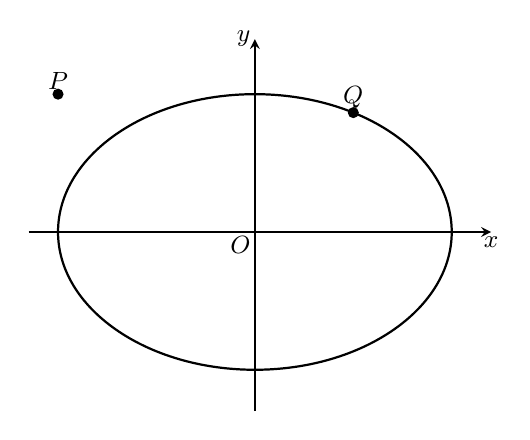
\begin{tikzpicture}[semithick, x=0.25cm, y=0.35cm, every node/.style={inner sep=1.3pt, font=\small}]
  \draw[-stealth] (-11.5,0) -- (12,0) node[below] {$x$};
  \draw[-stealth] (0,-6.5) -- (0,7) node[left] {$y$};
  \node[below left] at (0,0) {$O$};
  \draw[thick] (0,0) ellipse (10 and 5);
  \coordinate (P) at (-10,5);
  \coordinate (Q) at (5,4.330);
  \fill (P) circle (2pt);
  \fill (Q) circle (2pt);
  \node[above] at (P) {$P$};
  \node[above] at (Q) {$Q$};
\end{tikzpicture}
